\documentclass[accentcolor=tud4c,colorbacktitle]{tudbeamer}

\usepackage{ngerman}
\usepackage[utf8]{inputenc}
\usepackage{graphicx}

\title{Entwicklung eines adaptiven Chat-Systems}
\author{Johannes Lauinger, Jonas Mönnig, Matthias Hofmann, Max Weller, Simon-Konstantin Thiem}

\begin{document}

  \begin{titleframe}
    \textbf{Team:}\\
    Johannes Lauinger, Jonas Mönnig, Matthias Hofmann, Max Weller, Simon-Konstantin Thiem\\
    \vspace{0.5cm}
    \textbf{Teamleiter:}\\
    Benjamin Tumele
  \end{titleframe}

  \begin{frame}
    \frametitle{Was ist BonfireChat?}
    \begin{itemize}
      \item Hybride Chat-Anwendung: Peer-to-peer und Internet
      \item Bluetooth und WiFi Direct
      \item Routing durch AdHoc-Mesh-Netzwerk
      \item Kontaktaustausch dezentral: NFC, QR-Codes, Internet als Fallback
      \item Android App
    \end{itemize}
  \end{frame}

  \begin{frame}
    \frametitle{Projektfortschritt}
    \begin{itemize}
      \item GUI
      \item Datenbank
      \item Nachrichten verschicken über Bluetooth, WiFi Direct und Google Cloud Messaging
      \item Ende-zu-Ende-Verschlüsselung
      \item Kontaktdaten austauschen
      \item Flooding der Nachrichten
      \item Dashboard mit Statistiken
    \end{itemize}
  \end{frame}

  \begin{frame}
    \frametitle{Umsetzbarkeit}
    \begin{itemize}
      \item intelligentes Routing
      \item Energieeffizienz
      \item unterstützte Technologie der Handys
    \end{itemize}
    \begin{itemize}
      \item insgesamt voraussichtlich umsetzbar
    \end{itemize}
  \end{frame}

  \begin{frame}
    \frametitle{User Interface}
  \end{frame}

  \begin{frame}
    \frametitle{Qualitätsziele}
    \begin{itemize}
      \item Wartbarkeit durch Codequalität
      \item Korrektheit
      \item Robustheit
    \end{itemize}
  \end{frame}

  \begin{frame}
    \frametitle{Wartbarkeit durch Codequalität}
    \begin{itemize}
      \item Auftraggeber werden die App weiterentwickeln
      \item Einsatz beim Schlossgrabenfest 2016
    \end{itemize}
    \begin{itemize}
      \item Maßnahmen:
        \begin{itemize}
          \item Checkstyle: automatische Berichte
          \item Code Reviews
          \item technische Dokumentation
        \end{itemize}
    \end{itemize}
  \end{frame}

  \begin{frame}
    \frametitle{Korrektheit}
    \begin{itemize}
      \item Benutzer erwarten korrekte Zustellung ihrer Nachrichten
      \item Ende-zu-Ende-Verschlüsselung
      \item lokale Speicherung
    \end{itemize}
    \begin{itemize}
      \item Maßnahmen:
        \begin{itemize}
          \item automatisierte JUnit Tests
          \item FindBugs
        \end{itemize}
    \end{itemize}
  \end{frame}

  \begin{frame}
    \frametitle{Robustheit}
    \begin{itemize}
      \item für außergewöhnliche Situationen entwickelt
      \item hohe Fehlertoleranz
      \item Sonderfälle beachten
    \end{itemize}
    \begin{itemize}
      \item Maßnahmen: regelmäßige manuelle Tests
    \end{itemize}
  \end{frame}

  \begin{frame}
    \frametitle{aufgewendete Arbeitszeit}
    \begin{center}
      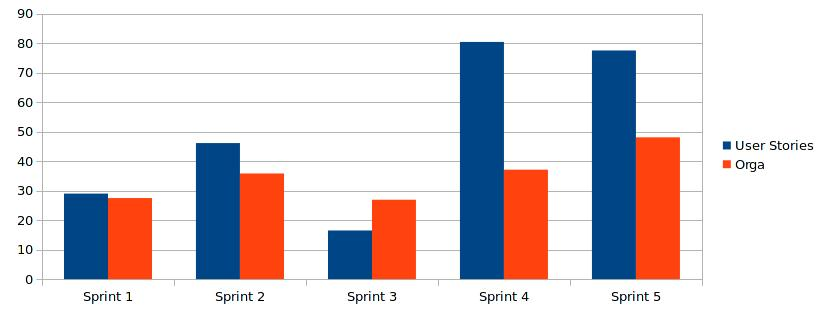
\includegraphics[height=4.5cm]{zeiten.jpg}
    \end{center}
  \end{frame}

  \begin{frame}
    \frametitle{aufgewendete Arbeitszeit}
    \begin{center}
      \huge{Insgesamt: 393 Stunden}
      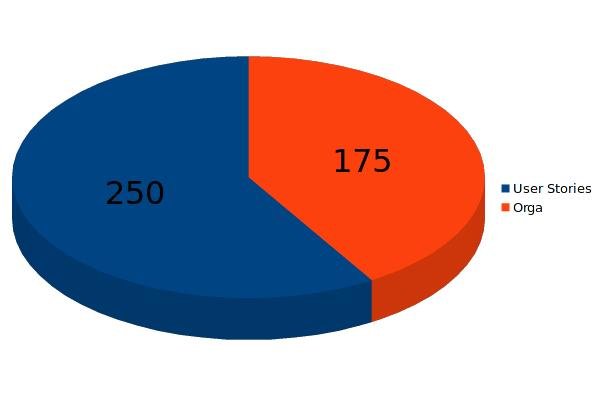
\includegraphics[height=5cm]{zeiten2.jpg}
    \end{center}
  \end{frame}


  \begin{frame}
    \frametitle{Danke für die Aufmerksamkeit!}
    \vspace{2cm}
    \begin{center}
      \huge{Fragen \& Antworten}
    \end{center}
  \end{frame}

\end{document}
